\chapter{Chemical Reactions: Reactants and Products}\label{ch:g7:chemical-reactions}

Charcoal glows in a barbecue. An hour later almost nothing is left of
the black lumps --- a little grey ash, and the heat that cooked the
meal. Where has the black carbon gone? It has not vanished: it has met
the oxygen of the \omterm{def:g4:air-a-mixture-of-gases:air}{air} and become a new, invisible gas. With \omterm{def:g7:atoms-and-molecules:atom}{atoms} and
\omterm{def:g7:atoms-and-molecules:molecule}{molecules} in hand, we can now say exactly what happens in such a change.

\begin{recall}
In a \omterm{def:g5:irreversible-changes:chemical-change}{chemical change} new substances appear and there is no simple way
back (\cref{ch:g5:irreversible-changes}). Limewater turns milky with
carbon dioxide, anhydrous copper sulfate turns blue with water
(\cref{ch:g7:identifying-substances}). All matter is made of \omterm{def:g7:atoms-and-molecules:atom}{atoms},
which group into \omterm{def:g7:atoms-and-molecules:molecule}{molecules}; a formula such as \ce{CO2} lists the \omterm{def:g7:atoms-and-molecules:atom}{atoms} of
a \omterm{def:g7:atoms-and-molecules:molecule}{molecule} (\cref{ch:g7:atoms-and-molecules}).
\end{recall}

\begin{omfigure}
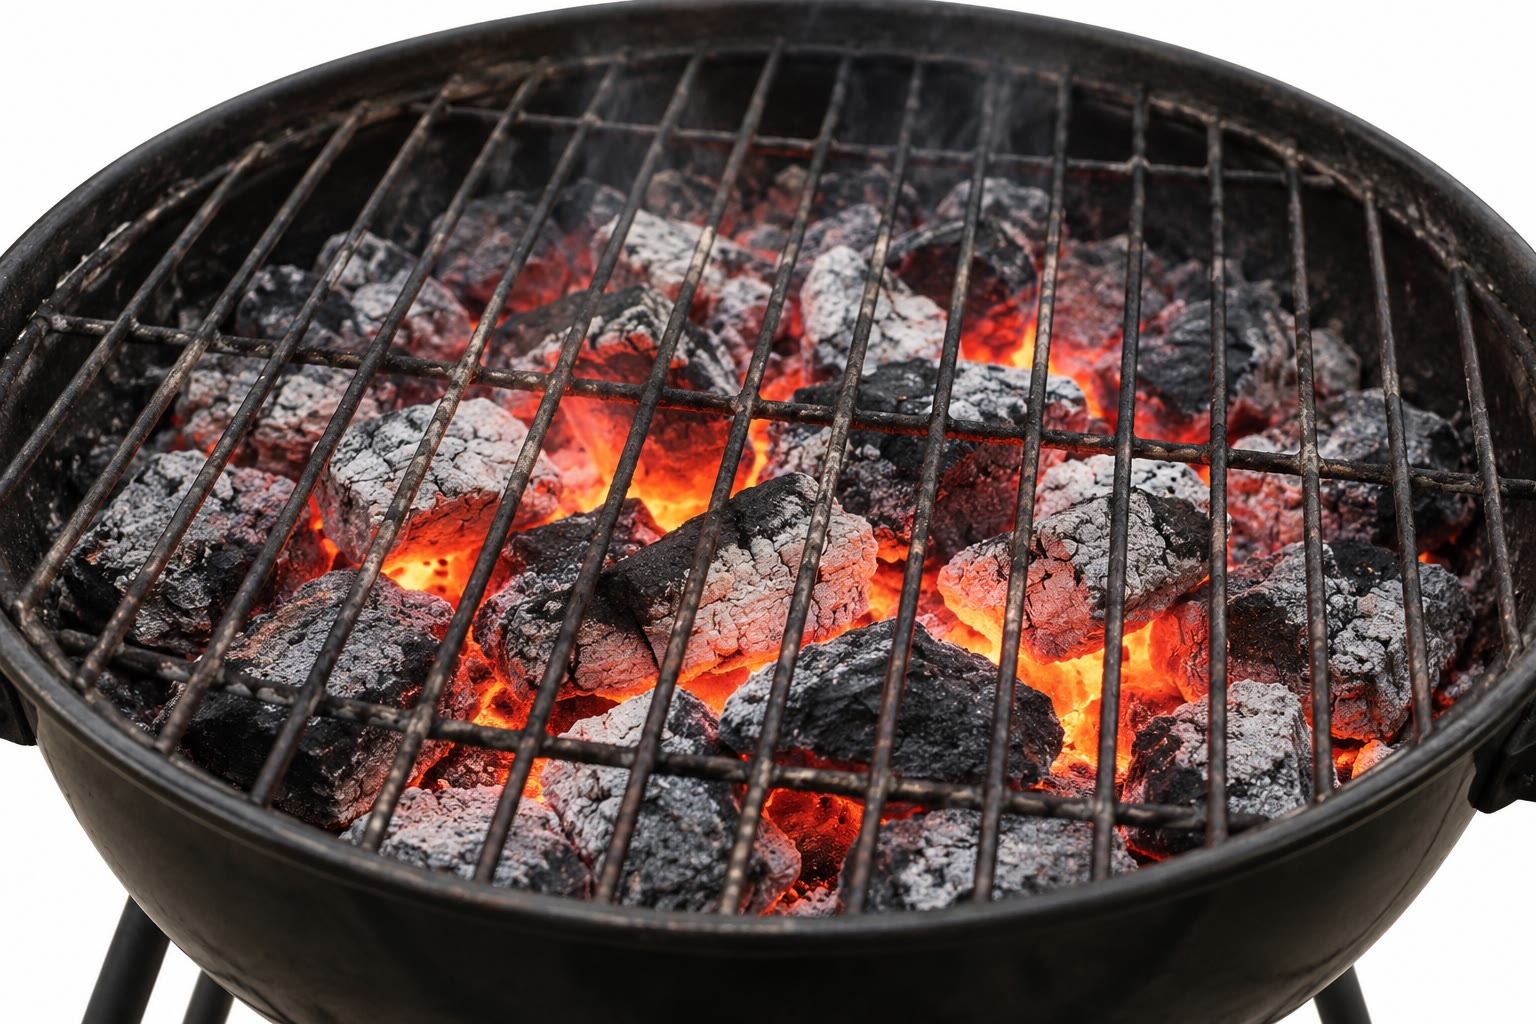
\includegraphics[width=0.55\linewidth]{images/book1/ai/g7-charcoal-bbq.jpg}

{\small Glowing charcoal: carbon reacting with the oxygen of the \omterm{def:g4:air-a-mixture-of-gases:air}{air}.}
\end{omfigure}

\section{Physical and chemical transformations}

\begin{definition}[Physical transformation]\label{def:g7:chemical-reactions:physical-transformation}
A \emph{physical transformation}\index{physical transformation} changes
the state or the arrangement of matter without changing the \omterm{def:g6:pure-substances-and-mixtures:species}{chemical
species}: melting, freezing, boiling, dissolving, mixing. The same
species are present before and after; only their form or their
arrangement has changed.
\end{definition}

\begin{example}[Water, three ways]\label{ex:g7:chemical-reactions:water}
Ice melting into water, water boiling into water vapour, and salt
dissolving in water are \omterm{def:g7:chemical-reactions:physical-transformation}{physical transformations}: before and after,
there are water \omterm{def:g7:atoms-and-molecules:molecule}{molecules} (and salt). Zooming in, the \omterm{def:g7:atoms-and-molecules:molecule}{molecules} are the
same; only how they are arranged and how they move has changed.
\end{example}

\begin{proposition}[Chemical transformation]\label{prop:g7:chemical-reactions:chemical}
In a \omterm{def:g5:irreversible-changes:chemical-change}{chemical change}, also called a chemical transformation, some
\omterm{def:g6:pure-substances-and-mixtures:species}{chemical species} disappear and new ones appear. It is told apart from a
\omterm{def:g7:chemical-reactions:physical-transformation}{physical transformation} by its \omterm{def:g7:chemical-reactions:reactant}{products}: new species, which can be
detected with \omterm{def:g7:identifying-substances:characteristic-test}{characteristic tests}.
\end{proposition}

\begin{omfigure}
\begin{tikzpicture}[font=\small, level distance=1.5cm,
    box/.style={draw=omDef, fill=omDef!6, rounded corners=2pt, align=center,
      inner sep=4pt},
    level 1/.style={sibling distance=6.6cm},
    edge from parent/.style={draw, thick, omDef, ->}]
  \node[box] {a transformation of matter}
    child {node[box, text width=5.2cm] {\textbf{physical}: the same species\\
      before and after\\ \footnotesize melting, boiling, dissolving, mixing}}
    child {node[box, draw=omProp, fill=omProp!6, text width=5.2cm]
      {\textbf{chemical}: species disappear,\\ new species appear\\
      \footnotesize burning, rusting, cooking}};
\end{tikzpicture}

{\small Two kinds of transformation.}
\end{omfigure}

\section{Reactants and products}

\begin{definition}[Chemical reaction]\label{def:g7:chemical-reactions:reaction}
A \emph{chemical reaction}\index{chemical reaction} is the model chemists
use for a chemical transformation: it lists the species that are used up
and the species that are formed.
\end{definition}

\begin{definition}[Reactants and products]\label{def:g7:chemical-reactions:reactant}
The species used up in a \omterm{def:g7:chemical-reactions:reaction}{chemical reaction} are the
\emph{reactants}\index{reactant}; the species formed are the
\emph{products}\index{product}.
\end{definition}

\begin{example}[Carbon burning in oxygen]\label{ex:g7:chemical-reactions:carbon}
When charcoal burns, the \omterm{def:g7:chemical-reactions:reactant}{reactants} are carbon (the charcoal) and oxygen
(from the \omterm{def:g4:air-a-mixture-of-gases:air}{air}). The \omterm{def:g7:chemical-reactions:reactant}{product} is carbon dioxide: shaken with limewater, the
gas left in the jar turns it milky.
\end{example}

\begin{inthelab}[Charcoal in a jar of oxygen]
The teacher heats a small piece of charcoal until it glows, on a
deflagrating spoon, then lowers it into a jar of oxygen. The charcoal
glows far brighter than in \omterm{def:g4:air-a-mixture-of-gases:air}{air} and shrinks until it has gone. The jar is
covered, a little limewater is poured in and shaken: it turns milky.
Carbon and oxygen have been used up; carbon dioxide has been formed.
\end{inthelab}

\begin{omfigure}
\begin{tikzpicture}[font=\small, scale=1.3]
  \pic[transform shape] at (0,0) {gasjaropen={0}{white}};
  \fill[omWater!60] (-0.68,2.62) rectangle (0.68,2.7);
  \draw[omGlass, line width=0.4pt] (-0.68,2.62) rectangle (0.68,2.7);
  \draw[black!60, line width=1.2pt] (0.15,2.7) -- (0.15,3.6) -- (1.2,3.6);
  \draw[black!60, line width=1.2pt] (0.15,2.7) -- (0.15,1.2);
  \fill[black!60] (-0.12,1.12) rectangle (0.32,1.2);
  \fill[red!70!black] (0.0,1.32) circle (0.13);
  \fill[orange!90!yellow] (0.0,1.32) circle (0.08);
  \draw[<-, omProp, thick] (0.15,1.35) -- (1.5,1.6) node[right, text=black]
    {glowing charcoal (carbon)};
  \draw[<-, omProp, thick] (-0.35,2.1) -- (1.5,2.3) node[right, text=black]
    {oxygen};
  \draw[<-, omProp, thick] (0.6,2.66) -- (1.5,2.95) node[right, text=black]
    {cover};
  \draw[<-, omProp, thick] (0.15,3.1) -- (1.5,3.6) node[right, text=black]
    {deflagrating spoon};
\end{tikzpicture}

{\small Glowing charcoal lowered on a spoon into a jar of oxygen burns
brightly: carbon and oxygen react to form carbon dioxide.}
\end{omfigure}

\begin{example}[Steel wool]\label{ex:g7:chemical-reactions:steel-wool}
A pad of fine steel wool, which is mostly iron, can burn in \omterm{def:g4:air-a-mixture-of-gases:air}{air} with
showers of sparks. The \omterm{def:g7:chemical-reactions:reactant}{reactants} are iron and oxygen; the \omterm{def:g7:chemical-reactions:reactant}{product} is a
dark, crumbly solid, an iron oxide.
\end{example}

\begin{omfigure}
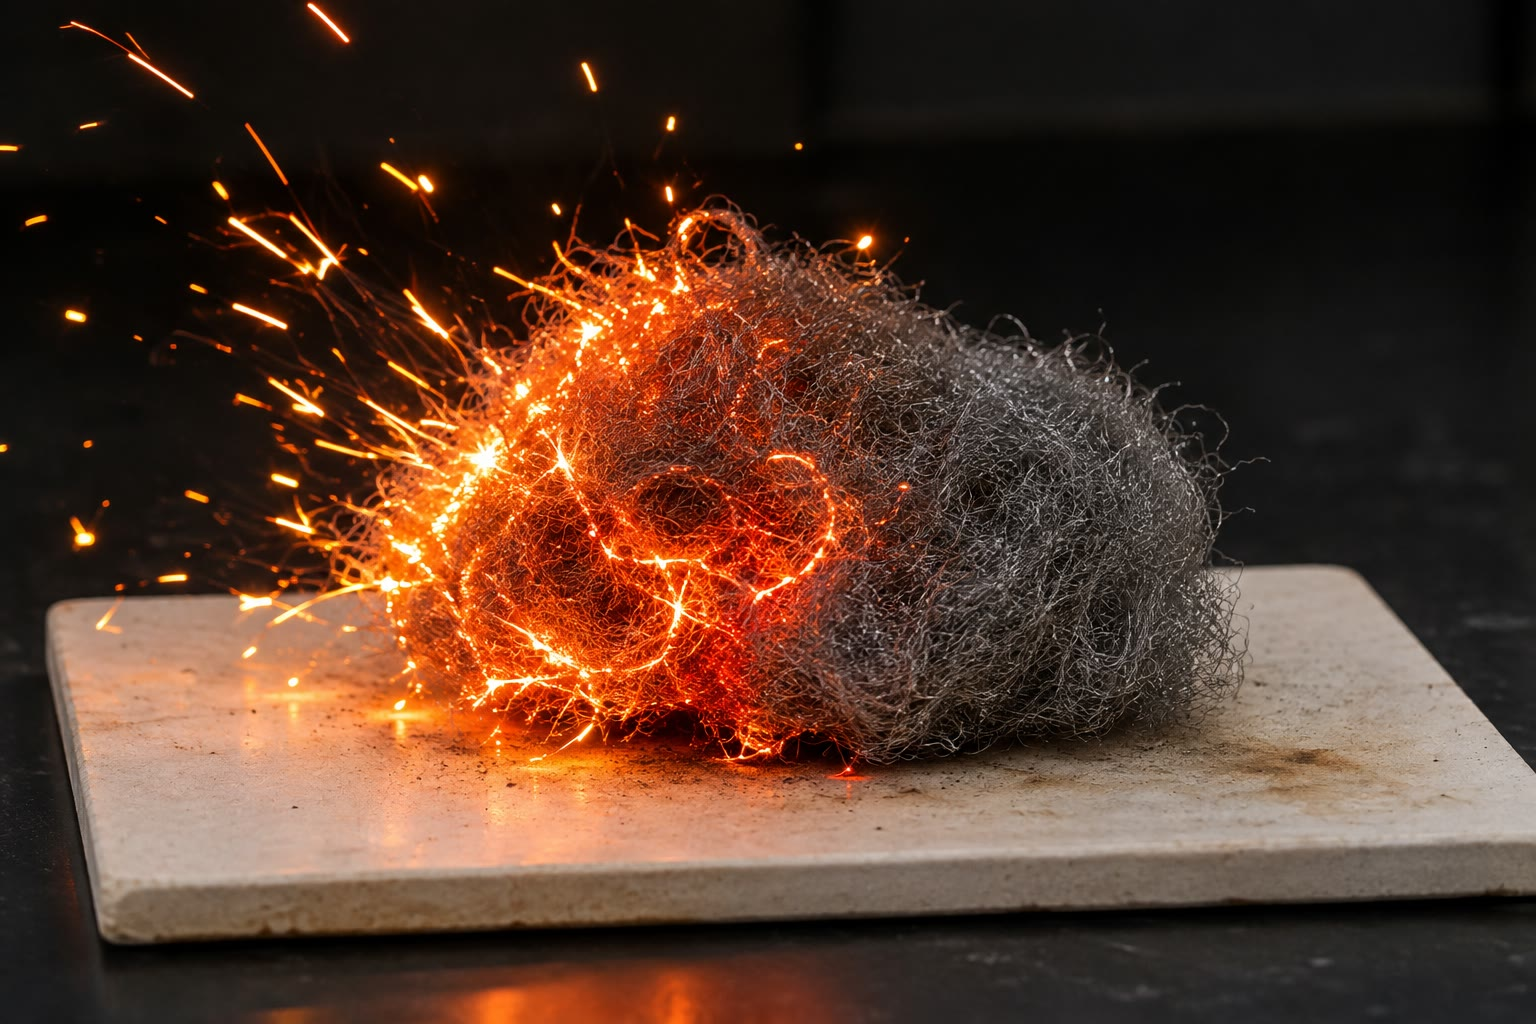
\includegraphics[width=0.5\linewidth]{images/book1/ai/g7-steel-wool-burning.jpg}

{\small Steel wool \omterm{def:g4:what-a-fire-needs:burning}{burning} in the laboratory: iron and oxygen react.}
\end{omfigure}

\section{The word equation}

\begin{definition}[Word equation]\label{def:g7:chemical-reactions:word-equation}
A \emph{word equation}\index{word equation} writes a \omterm{def:g7:chemical-reactions:reaction}{chemical reaction}
in words: the names of the \omterm{def:g7:chemical-reactions:reactant}{reactants} on the left, joined by $+$, an
arrow, and the names of the \omterm{def:g7:chemical-reactions:reactant}{products} on the right. The arrow reads
``react to give''.
\end{definition}

\begin{example}[Three word equations]\label{ex:g7:chemical-reactions:three}
\begin{center}
\begin{tabular}{l}
carbon $+$ oxygen $\longrightarrow$ carbon dioxide\\[2pt]
methane $+$ oxygen $\longrightarrow$ carbon dioxide $+$ water\\[2pt]
iron $+$ oxygen $\longrightarrow$ iron oxide
\end{tabular}
\end{center}
\end{example}

\begin{method}[Writing a word equation]\label{met:g7:chemical-reactions:write}
\begin{enumerate}
  \item Find the \omterm{def:g7:chemical-reactions:reactant}{reactants}: the species that disappear.
  \item Find the \omterm{def:g7:chemical-reactions:reactant}{products}: the new species, identified by tests.
  \item Write the \omterm{def:g7:chemical-reactions:reactant}{reactants} on the left, the \omterm{def:g7:chemical-reactions:reactant}{products} on the right,
        with an arrow between them; never an equals sign.
\end{enumerate}
A species that is present but takes no part --- the nitrogen of the \omterm{def:g4:air-a-mixture-of-gases:air}{air}
around a flame --- is not written.
\end{method}

\section{A reaction is a rearrangement of atoms}

\begin{proposition}[Atoms are rearranged]\label{prop:g7:chemical-reactions:rearranged}
In a \omterm{def:g7:chemical-reactions:reaction}{chemical reaction} the \omterm{def:g7:atoms-and-molecules:molecule}{molecules} of the \omterm{def:g7:chemical-reactions:reactant}{reactants} are broken apart
and their \omterm{def:g7:atoms-and-molecules:atom}{atoms} join up differently to build the \omterm{def:g7:atoms-and-molecules:molecule}{molecules} of the
\omterm{def:g7:chemical-reactions:reactant}{products}. The \omterm{def:g7:atoms-and-molecules:atom}{atoms} themselves are neither created nor destroyed: the
same \omterm{def:g7:atoms-and-molecules:atom}{atoms}, in the same numbers, are there before and after.
\end{proposition}

\begin{example}[Methane burning, molecule by molecule]\label{ex:g7:chemical-reactions:methane}
When the methane of a gas cooker burns, one methane \omterm{def:g7:atoms-and-molecules:molecule}{molecule} \ce{CH4}
meets two oxygen \omterm{def:g7:atoms-and-molecules:molecule}{molecules} \ce{O2}. Their \omterm{def:g7:atoms-and-molecules:atom}{atoms} rearrange into one
carbon dioxide \omterm{def:g7:atoms-and-molecules:molecule}{molecule} \ce{CO2} and two water \omterm{def:g7:atoms-and-molecules:molecule}{molecules} \ce{H2O}.
Before: 1 carbon, 4 hydrogen and 4 oxygen \omterm{def:g7:atoms-and-molecules:atom}{atoms}. After: 1 carbon, 4
hydrogen, and $2 + 2 = 4$ oxygen \omterm{def:g7:atoms-and-molecules:atom}{atoms}. Nothing is lost, nothing
appears from nowhere.
\end{example}

\begin{omfigure}
\begin{tikzpicture}[font=\small]
  % methane
  \begin{scope}[xshift=0cm]
    \node[aC] (c) at (0,0) {};
    \node[aH] (h1) at (0,0.78) {}; \node[aH] (h2) at (-0.74,-0.3) {};
    \node[aH] (h3) at (0.74,-0.3) {}; \node[aH] (h4) at (0.2,-0.68) {};
    \begin{scope}[on background layer]
      \foreach \h in {h1,h2,h3,h4} \draw[bond] (c.center) -- (\h.center);
    \end{scope}
    \node at (0,-1.2) {1 methane};
  \end{scope}
  \node at (1.45,0) {$+$};
  % two oxygen molecules
  \foreach \y in {0.45,-0.45} {
    \node[aO] (a) at (2.4,\y) {}; \node[aO] (b) at (3.05,\y) {};
    \begin{scope}[on background layer]
      \draw[bond, line width=1.1pt] ([yshift=1.6pt]a.center) -- ([yshift=1.6pt]b.center);
      \draw[bond, line width=1.1pt] ([yshift=-1.6pt]a.center) -- ([yshift=-1.6pt]b.center);
    \end{scope}
  }
  \node at (2.72,-1.2) {2 oxygen};
  \draw[->, thick, omProp] (3.8,0) -- (5.0,0);
  % carbon dioxide
  \begin{scope}[xshift=6.3cm]
    \node[aO] (a) at (-0.8,0) {}; \node[aC] (c) at (0,0) {}; \node[aO] (b) at (0.8,0) {};
    \begin{scope}[on background layer]
      \foreach \d in {-1.6,1.6} {
        \draw[bond, line width=1.1pt] ([yshift=\d pt]a.center) -- ([yshift=\d pt]c.center);
        \draw[bond, line width=1.1pt] ([yshift=\d pt]c.center) -- ([yshift=\d pt]b.center);}
    \end{scope}
    \node at (0,-1.2) {1 carbon dioxide};
  \end{scope}
  \node at (7.8,0) {$+$};
  % two water molecules
  \foreach \x in {8.9,10.6} {
    \node[aO] (o) at (\x,0.2) {};
    \node[aH] (p) at (\x-0.58,-0.25) {}; \node[aH] (q) at (\x+0.58,-0.25) {};
    \begin{scope}[on background layer]
      \draw[bond] (o.center) -- (p.center); \draw[bond] (o.center) -- (q.center);
    \end{scope}
  }
  \node at (9.75,-1.2) {2 water};
  % atom counts
  \node[align=center, font=\footnotesize] at (1.5,-2.0) {before: 1 C, 4 H, 4 O};
  \node[align=center, font=\footnotesize] at (8.5,-2.0) {after: 1 C, 4 H, 4 O};
\end{tikzpicture}

{\small Methane \omterm{def:g4:what-a-fire-needs:burning}{burning}, drawn with molecular models: the \omterm{def:g7:atoms-and-molecules:atom}{atoms} of the
\omterm{def:g7:chemical-reactions:reactant}{reactants} rearrange into the \omterm{def:g7:chemical-reactions:reactant}{products}. The same \omterm{def:g7:atoms-and-molecules:atom}{atoms} are counted before
and after.}
\end{omfigure}

\begin{remark}[Counting the molecules]\label{rem:g7:chemical-reactions:counting}
The \omterm{def:g7:chemical-reactions:word-equation}{word equation} does not say how many \omterm{def:g7:atoms-and-molecules:molecule}{molecules} react: for that, the
equation is written with formulas and numbers in front of them. Writing
such equations, and finding the right numbers, is the subject of a
later chapter.
\end{remark}

\section{Exercises}

\begin{exercise}[$\star$]\label{exo:g7:chemical-reactions:1}
Physical or chemical transformation? Ice melting, a match \omterm{def:g4:what-a-fire-needs:burning}{burning}, sugar
dissolving, bread toasting, a nail rusting.
\end{exercise}

\begin{exercise}[$\star$]\label{exo:g7:chemical-reactions:2}
What are the \omterm{def:g7:chemical-reactions:reactant}{reactants} and the \omterm{def:g7:chemical-reactions:reactant}{products} of a \omterm{def:g7:chemical-reactions:reaction}{chemical reaction}?
\end{exercise}

\begin{exercise}[$\star$]\label{exo:g7:chemical-reactions:3}
Write the \omterm{def:g7:chemical-reactions:word-equation}{word equation} of the \omterm{def:g4:what-a-fire-needs:burning}{burning} of carbon in oxygen.
\end{exercise}

\begin{exercise}[$\star$]\label{exo:g7:chemical-reactions:4}
In the \omterm{def:g7:chemical-reactions:word-equation}{word equation} ``iron $+$ oxygen $\longrightarrow$ iron oxide'',
name the \omterm{def:g7:chemical-reactions:reactant}{reactants} and the \omterm{def:g7:chemical-reactions:reactant}{product}.
\end{exercise}

\begin{exercise}[$\star\star$]\label{exo:g7:chemical-reactions:5}
When methane burns, a cold glass held above the flame mists up, and the
gas collected turns limewater milky. Which \omterm{def:g7:chemical-reactions:reactant}{products} do these two tests
show?
\end{exercise}

\begin{exercise}[$\star\star$]\label{exo:g7:chemical-reactions:6}
Zinc reacts with hydrochloric acid: the zinc disappears, bubbles of
hydrogen are given off, and zinc chloride stays in the solution. Write
the \omterm{def:g7:chemical-reactions:word-equation}{word equation}.
\end{exercise}

\begin{exercise}[$\star\star$]\label{exo:g7:chemical-reactions:7}
Look at the model figure of methane \omterm{def:g4:what-a-fire-needs:burning}{burning}. Count the hydrogen \omterm{def:g7:atoms-and-molecules:atom}{atoms}
before and after the reaction.
\end{exercise}

\begin{exercise}[$\star\star$]\label{exo:g7:chemical-reactions:8}
Why is dissolving salt in water not a \omterm{def:g7:chemical-reactions:reaction}{chemical reaction}, although the
salt disappears from sight?
\end{exercise}

\begin{exercise}[$\star\star$]\label{exo:g7:chemical-reactions:9}
A log of wood burns down to a small heap of ash. Explain, using the word
``\omterm{def:g7:chemical-reactions:reactant}{products}'', why the ash is so much lighter than the log.
\end{exercise}

\begin{exercise}[$\star\star$]\label{exo:g7:chemical-reactions:10}
Hydrogen burns in oxygen to give water only. Write the \omterm{def:g7:chemical-reactions:word-equation}{word equation},
and say which test would identify the \omterm{def:g7:chemical-reactions:reactant}{product}.
\end{exercise}

\begin{exercise}[$\star\star\star$]\label{exo:g7:chemical-reactions:11}
Two hydrogen \omterm{def:g7:atoms-and-molecules:molecule}{molecules} \ce{H2} react with one oxygen \omterm{def:g7:atoms-and-molecules:molecule}{molecule} \ce{O2} to
give two water \omterm{def:g7:atoms-and-molecules:molecule}{molecules} \ce{H2O}. Count the \omterm{def:g7:atoms-and-molecules:atom}{atoms} of each kind before
and after, and show that none has been created or destroyed.
\end{exercise}

\begin{exercise}[$\star\star\star$]\label{exo:g7:chemical-reactions:12}
A student draws the \omterm{def:g4:what-a-fire-needs:burning}{burning} of carbon as: one carbon \omterm{def:g7:atoms-and-molecules:atom}{atom} $+$ one oxygen
\omterm{def:g7:atoms-and-molecules:molecule}{molecule} $\longrightarrow$ one carbon dioxide \omterm{def:g7:atoms-and-molecules:molecule}{molecule} and one oxygen
\omterm{def:g7:atoms-and-molecules:atom}{atom} left over. What is wrong with this drawing? Draw the correct one in
words.
\end{exercise}

\section{Problem: Inside a Gas-Cooker Flame}

\begin{problem}[{Weekend problem --- what burns in a gas-cooker flame, what
it makes, and how many molecules take part}]
\label{pb:g7:chemical-reactions:1}
The gas of a kitchen cooker is mostly methane, \ce{CH4}. In its blue
flame, methane reacts with the oxygen of the \omterm{def:g4:air-a-mixture-of-gases:air}{air}. In a laboratory, the
teacher holds a cold, dry beaker upside down above such a flame for a
few seconds, then turns it over, pours in a little limewater and shakes
it.

\medskip
\noindent\textbf{Part I --- \omterm{def:g7:chemical-reactions:reactant}{Reactants} and \omterm{def:g7:chemical-reactions:reactant}{products}.}
\begin{enumerate}
  \item Name the two \omterm{def:g7:chemical-reactions:reactant}{reactants} of this reaction.
  \item Droplets appear inside the cold beaker; a drop of them turns
        anhydrous copper sulfate blue. Which \omterm{def:g7:chemical-reactions:reactant}{product} does this show?
  \item The limewater turns milky. Which other \omterm{def:g7:chemical-reactions:reactant}{product} does this show?
  \item The \omterm{def:g4:air-a-mixture-of-gases:air}{air} also contains nitrogen, which passes through the flame
        unchanged. Is nitrogen a \omterm{def:g7:chemical-reactions:reactant}{reactant}? Should it appear in the \omterm{def:g7:chemical-reactions:word-equation}{word
        equation}?
\end{enumerate}

\medskip
\noindent\textbf{Part II --- The \omterm{def:g7:chemical-reactions:word-equation}{word equation}.}
\begin{enumerate}[resume]
  \item Write the \omterm{def:g7:chemical-reactions:word-equation}{word equation} of the reaction.
  \item Is the \omterm{def:g4:what-a-fire-needs:burning}{burning} of methane a physical or a chemical
        transformation? Give two reasons.
  \item Write the formulas of the four species of the reaction.
\end{enumerate}

\medskip
\noindent\textbf{Part III --- Counting \omterm{def:g7:atoms-and-molecules:molecule}{molecules}.}
Each methane \omterm{def:g7:atoms-and-molecules:molecule}{molecule} that burns reacts with two oxygen \omterm{def:g7:atoms-and-molecules:molecule}{molecules}, and
gives one carbon dioxide \omterm{def:g7:atoms-and-molecules:molecule}{molecule} and two water \omterm{def:g7:atoms-and-molecules:molecule}{molecules}.
\begin{enumerate}[resume]
  \item Count the carbon, hydrogen and oxygen \omterm{def:g7:atoms-and-molecules:atom}{atoms} in one methane
        \omterm{def:g7:atoms-and-molecules:molecule}{molecule} and two oxygen \omterm{def:g7:atoms-and-molecules:molecule}{molecules}, together.
  \item Count them in one carbon dioxide \omterm{def:g7:atoms-and-molecules:molecule}{molecule} and two water \omterm{def:g7:atoms-and-molecules:molecule}{molecules},
        together. What do you notice?
  \item The flame burns 10 methane \omterm{def:g7:atoms-and-molecules:molecule}{molecules}. How many oxygen \omterm{def:g7:atoms-and-molecules:molecule}{molecules}
        does it use?
  \item How many carbon dioxide \omterm{def:g7:atoms-and-molecules:molecule}{molecules} does it make?
  \item How many water \omterm{def:g7:atoms-and-molecules:molecule}{molecules} does it make?
\end{enumerate}
\end{problem}
